% Multiple Choice Question 15

\begin{center}
    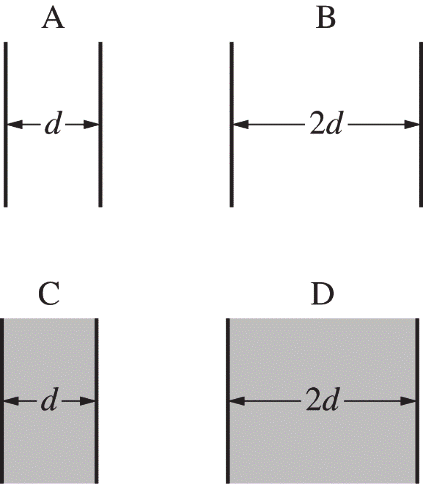
\includegraphics[scale=0.4]{images/img-007-008.png}
\end{center}

\begin{questions}
\setcounter{question}{14}

\question
Four parallel plate capacitors all have the same plate area and have the plate separations shown above. Both capacitors A and B have air between the plates, while the space between the plates of both capacitors C and D is filled with a dielectric slab of dielectric constant $\kappa=2$. Which of the following correctly ranks the capacitors in order of their capacitance from largest to smallest?

\begin{choices}
    \choice $\mathrm{B}>(\mathrm{A}=\mathrm{D})>\mathrm{C}$
    \choice $(\mathrm{A}=\mathrm{C})>(\mathrm{B}=\mathrm{D})$
    \choice $\mathrm{C}>(\mathrm{A}=\mathrm{D})>\mathrm{B}$
    \choice $(\mathrm{B}=\mathrm{D})>(\mathrm{A}=\mathrm{C})$
    \choice $\mathrm{D}>\mathrm{C}>\mathrm{B}>\mathrm{A}$
\end{choices}

\end{questions}
